\documentclass[12pt]{article}
\usepackage[utf8]{inputenc}
\usepackage[english]{babel}
\usepackage{subcaption}
\usepackage{graphicx}
\usepackage{geometry}
\usepackage{url}
\usepackage[hang,flushmargin]{footmisc}
\usepackage{fancyhdr}
\usepackage{lastpage}
\usepackage{footnote}
\usepackage{float}
\usepackage{textcomp}
\usepackage[colorinlistoftodos]{todonotes}
%\usepackage[hidelinks]{hyperref}
\PassOptionsToPackage{hyphens}{url}\usepackage{hyperref}
\hypersetup{colorlinks, linkcolor=black, urlcolor=blue}
\usepackage{listings}
\usepackage{color}
\usepackage{cleveref}

\definecolor{dkgreen}{rgb}{0,0.6,0}
\definecolor{gray}{rgb}{0.5,0.5,0.5}
\definecolor{mauve}{rgb}{0.58,0,0.82}

\lstset{frame=single,
	backgroundcolor = \color{lightgray},
	language=Java,
	aboveskip=3mm,
	belowskip=3mm,
	showstringspaces=false,
	columns=flexible,
	basicstyle={\small\ttfamily},
	numbers=none,
	numberstyle=\tiny\color{gray},
	keywordstyle=\color{blue},
	commentstyle=\color{dkgreen},
	stringstyle=\color{mauve},
	breaklines=true,
	breakatwhitespace=true,
	tabsize=3
}

%Layout di pagina
\geometry{
	a4paper,
	total={160mm,225mm},
	left=25mm,
	top=25mm
}

%intestazione e piè di pagina
\pagestyle{fancy}
\fancyhf{}
\renewcommand{\headrulewidth}{0.4pt}
\renewcommand{\footrulewidth}{0.4pt}
\setlength\headheight{57pt}
\lhead{Rendering-Report}
\lfoot{Rendering-Report}
\rfoot{Page \thepage\ of \pageref{LastPage}}

\newcommand\imagescale{0.5}
%\newcommand{\code}[1]{\texttt{#1}}
\interfootnotelinepenalty=10000
\DeclareTextFontCommand{\code}{\ttfamily\hyphenchar\font=45\relax}

\begin{document}
	\begin{titlepage} % Suppresses displaying the page number on the title page
	\begin{center} % Centre everything on the page

		%------------------------------------------------
		%	Headings
		%------------------------------------------------
		
		\textsc{\LARGE Denmark Technical University}\\[1.5cm]
		
		\textsc{\Large Rendering - Introduction}\\[0.5cm]
		
		\textsc{\large 2020/2021}\\[0.5cm] % Minor heading such as course title
		
		%------------------------------------------------
		%	Title
		%------------------------------------------------
		
		{\huge\ Report}\\[0.4cm] % Title of your document
		
		%------------------------------------------------
		%	Author(s)
		%------------------------------------------------
		
	 	\large
			\begin{tabular}{l r}
				Giacomo \textsc{Barzon} & 201434 \\
			\end{tabular}
	\end{center}
\end{titlepage}
	%----------------------------------------------------------------------------------------
	\section*{Introduction}
This is the final report of the course \textit{Rendering, Introduction - 02562}. Inside this document you will find the report for the exercises and the project combined.\\
Both the reports and the code of all exercises and the project was made individually by \textit{Barzon Giacomo - s201434}. I didn't participate in any group work for the entirety of this course.
	\tableofcontents
	\section{Worksheet 1}
The deafault rendering of the framework can be seen in figure \ref{fig:preview}.
\begin{figure}[H]
	\centering
	
\includegraphics[scale=\imagescale]{images/worksheet_1/preview}
	\caption{Default rendering}
	\label{fig:preview}
\end{figure}
The first thing we do is implementing the render function in the RenderEngine class which loops over all pixels. For now the compute\_pixel function returns only red pixels.
\begin{lstlisting}
void RenderEngine::render()
{
	cout << "Raytracing";
	Timer timer;
	timer.start();
	
	int x_res = static_cast<int>(res.x);
	int y_res = static_cast<int>(res.y);
	#pragma omp parallel for private(randomizer)
	for(int y = 0; y < y_res ; ++y)
	{
		for (int x = 0; x < x_res; ++x)
		{
			image[x+y*y_res] = tracer.compute_pixel(x, y);
		}
		if(((y + 1) % 50) == 0) 
		cerr << ".";
	}
	
	timer.stop();
	cout << " - " << timer.get_time() << " secs " << endl;
	init_texture();
	done = true;
}
\end{lstlisting}
Then we proceed to implementing the set, get\_ray\_dir and get\_ray direction that we can find in the Camera class.
\begin{lstlisting}
void Camera::set(const float3& eye_point, const float3& view_point, const float3& up_vector, float camera_constant)
{
	eye = eye_point;
	lookat = view_point;
	up = up_vector;
	cam_const = camera_constant;
	
	ip_normal = normalize(lookat - eye) ;
	ip_xaxis = normalize(cross(ip_normal, up));
	ip_yaxis = cross(ip_xaxis, ip_normal);
	
	float fov_rad = 2 * atan(1/(2 * cam_const));
	fov = fov_rad * 180 * M_1_PIf;
}

float3 Camera::get_ray_dir(const float2& coords) const{
	float3 q = ip_xaxis * coords.x + ip_yaxis * coords.y + ip_normal * cam_const;
	return normalize(q);
}

Ray Camera::get_ray(const float2& coords) const{
	float3 dir = get_ray_dir(coords);
	Ray r = Ray(eye, dir, 0,0, RT_DEFAULT_MAX);
	return r; 
}
\end{lstlisting}
Now we implement the closest\_hit function of the Accelerator class which will allow us to check the closest primitive to which our ray intersects to.
\begin{lstlisting}
bool Accelerator::closest_hit(optix::Ray& r, HitInfo& hit) const
{
	closest_plane(r, hit);
	
	for (unsigned int i = 0; i < primitives.size(); ++i)
		if (primitives[i]->geometry->intersect(r, hit, 0))
			r.tmax = hit.dist;
	return hit.has_hit;
}
\end{lstlisting}
Now we can implement the compute\_pixel function that we used before in the render function of RenderEngine.
\begin{lstlisting}
	float3 RayCaster::compute_pixel(unsigned int x, unsigned int y) const
	{
		Camera* camera = scene->get_camera();
		float2 coords = make_float2(lower_left.x + win_to_ip.x * x, lower_left.y + win_to_ip.y * y);
		float3 color = make_float3(0.0f);
		
		
		Ray ray = camera->get_ray(coords);
		
		HitInfo hit = HitInfo();
		bool has_hit = scene->closest_hit(ray, hit);
		if (has_hit) {
			color=color+ get_shader(hit)->shade(ray, hit);
		}
		else {
			color = color + get_background(ray.direction);
		}
		
		return color;
	}
\end{lstlisting}
After the previous step we should obtain a fully blue image, as the colour of the background, since the intersect function of our primitive objects isn't implemented yet. In our scene we have a sphere, a plane and a triangle. 
\begin{lstlisting}
bool Sphere::intersect(const Ray& r, HitInfo& hit, unsigned int prim_idx) const
{
	float b_half = dot((r.origin - center), r.direction);
	float c = dot((r.origin - center), (r.origin - center)) - (radius * radius);
	float t1 = -b_half - sqrt((b_half * b_half) - c);
	float t2 = -b_half + sqrt((b_half * b_half) - c);
	
	float min_t;
	if (t1 < t2) {
		min_t = t1;;
	}
	else {
		min_t = t2;
	}
	
	bool intersected = ((b_half * b_half) - c) > 0;
	bool has_hit=  intersected && min_t>r.tmin && min_t<r.tmax;
	float3 normal = normalize(hit.position-center);
	if (has_hit) {
		hit.has_hit = true;
		hit.dist = min_t;
		hit.material = &material;
		hit.geometric_normal = normal;
		hit.shading_normal = normal;
		hit.position = r.origin + r.direction * hit.dist;
	}
	return has_hit;
}

bool intersect_triangle(const Ray& ray, const float3& v0, const float3& v1, 
const float3& v2, float3& n,float& t,float& v,float& w)
{
	float3 e0 = v1 - v0;
	float3 e1 = v0 - v2;
	n = cross(e0, e1);
	float d = dot(-v0, n);
	t = dot((v0 - ray.origin), n) / dot(ray.direction, n);
	
	v = dot(cross((v0 - ray.origin), ray.direction), e1)/dot(ray.direction,n);
	w =  dot(cross((v0 - ray.origin), ray.direction), e0) / dot(ray.direction, n);
	float u = 1 - v - w;
	bool on_plane = dot(ray.direction, n) != 0;
	bool inside_triangle = v >= 0 && w >= 0 && v + w <= 1;
	bool has_hit = on_plane && inside_triangle && t > ray.tmin && t < ray.tmax;
	return has_hit;
}


bool Triangle::intersect(const Ray& r, HitInfo& hit, unsigned int prim_idx) const
{
	float3 n;
	float t;
	float v;
	float w;
	bool has_hit=::intersect_triangle(r,v0,v1,v2,n,t,v,w);
	
	if (has_hit) {
		hit.has_hit = true;
		hit.dist = t;
		hit.geometric_normal = -normalize(n);
		hit.shading_normal = -normalize(n);
		hit.material = &material;
		hit.position = r.origin + r.direction * hit.dist;
	}
	return has_hit;
}

bool Plane::intersect(const Ray& r, HitInfo& hit, unsigned int prim_idx) const
{
	float t1 = -(dot(r.origin, onb.m_normal) + d) / dot(r.direction, onb.m_normal);
	bool intersect = dot(r.direction, onb.m_normal) != 0;
	bool has_hit =  intersect && t1 > r.tmin && t1 < r.tmax;
	if (has_hit){
		hit.has_hit = true;
		hit.dist = t1;
		hit.position = r.origin + (r.direction * t1);
		hit.geometric_normal = normalize(onb.m_normal);
		hit.shading_normal = normalize(onb.m_normal);
		hit.material = &material;
	}
	return has_hit;
}
\end{lstlisting}
Now that we have implemented all of the core methods of our ray tracing framework we can see a render of the image which is really similar to default one like the one that can be seen in figure \ref{fig:default_shading}.
\begin{figure}[H]
	\centering
	
\includegraphics[scale=\imagescale]{images/worksheet_1/default_shading}
	\caption{RayTracing with default shading}
	\label{fig:default_shading}
\end{figure}
The results is almost identical to the one that we can see in the preview, the only differnece is that some of the aliasing artifacts present at the end of the plane have disappeared.\\
Now we implement lambertian shading by implementing the function PointLight::sample and the function Lambertian::shade. 
\begin{lstlisting}
bool PointLight::sample(const float3& pos, float3& dir, float3& L) const
{	
	dir = light_pos - pos;
	L = intensity / sqrt(pow(dir.x, 2) + pow(dir.y, 2) + pow(dir.z, 2));
	return false;
}

float3 Lambertian::shade(const Ray& r, HitInfo& hit, bool emit) const
{
	float3 rho_d = get_diffuse(hit);
	float3 result = make_float3(0.0f);

	for (int i = 0; i < lights.size();i++) {
		float3 dir;
		float3 L;
		
		bool shade=lights[i]->sample(hit.position, dir, L);
		if (dot(dir, hit.shading_normal) > 0) {
			result = result + (rho_d / M_PIf) * L * (dot(dir, hit.shading_normal));
		}
	}
	return result + Emission::shade(r, hit, emit);
}
\end{lstlisting}
\begin{figure}[H]
	\centering
	
\includegraphics[scale=\imagescale]{images/worksheet_1/shading_of_diffuse_objects}
	\caption{}
	\label{fig:diffuse_shading}
\end{figure}
	\section{Worksheet 2}

\subsection{Ray Tracing}
We modify the function PointLight::Sample in order to implement hard shadows.
\begin{lstlisting}
bool PointLight::sample(const float3& pos, float3& dir, float3& L) const
{		
	dir = light_pos - pos;
	float dir_norm = length(dir);
	dir = normalize(dir);
	
	//Worksheet2 - point 1
	float epsilon = 1e-4;
	float cutoff_distance = dir_norm-epsilon;
	
	Ray shadow_ray = Ray(pos,dir,0,epsilon, RT_DEFAULT_MAX);
	HitInfo hit_info = HitInfo();
	
	tracer->trace_to_any(shadow_ray, hit_info);
	if (!hit_info.has_hit) {
		L = intensity / (dir_norm*dir_norm);
		
	}
	return !hit_info.has_hit;
}
\end{lstlisting}
\begin{figure}[H]
	\centering
	
\includegraphics[scale=\imagescale]{images/worksheet_2/part_1}
	\caption{Hard shadows}
	\label{fig:hard_shadows}
\end{figure}
We want to render our sphere with a glossy material which is a mixture of between a transparent and mirror-like material. To do that we have to implement first both the shading of mirror-like and transparent materials.\\
we start first with mirror shading.
\begin{lstlisting}
bool RayTracer::trace_reflected(const Ray& in, const HitInfo& in_hit, Ray& out, HitInfo& out_hit) const
{
	float3 out_direction=reflect(in.direction, in_hit.shading_normal);
	out = Ray(in_hit.position, out_direction,0,1e-4, RT_DEFAULT_MAX);
	trace_to_closest(out, out_hit);
	float3 normal;
	out_hit.ray_ior = in_hit.ray_ior;
	out_hit.trace_depth = in_hit.trace_depth + 1;
	return out_hit.has_hit;
}

float3 Glossy::shade(const Ray& r, HitInfo& hit, bool emit) const
{
	Mirror::shade(r, hit, emit);
}
\end{lstlisting}
Then we can move to transparent shading.
\begin{figure}[H]
	\centering
	
\includegraphics[scale=\imagescale]{images/worksheet_2/part_2}
	\caption{Mirror Reflections}
	\label{fig:mirror_reflections}
\end{figure}

\begin{lstlisting}
bool RayTracer::trace_refracted(const Ray& in, const HitInfo& in_hit, Ray& out, HitInfo& out_hit) const
{
	float3 normal;
	float out_ior = get_ior_out(in,in_hit,normal);
	out_hit.ray_ior = out_ior;
	bool refraction=refract(out.direction, in.direction, normal, out_hit.ray_ior / in_hit.ray_ior);
	if (refraction) {
		out.origin = in_hit.position;
		out.tmin = 1e-4;
		out.tmax = RT_DEFAULT_MAX;
		out_hit.trace_depth = in_hit.trace_depth + 1;
		
		trace_to_closest(out, out_hit);
		return out_hit.has_hit;
	}
	return refraction;
}

float3 Glossy::shade(const Ray& r, HitInfo& hit, bool emit) const
{
	Transparent::shade(r, hit, emit);
}
\end{lstlisting}
The function RayTracer::get\_ior\_out takes checks if the ray given in input hits an object, if it does then it returns the index of refraction of such material otherwise returns the index of refraction of the air which is 1.
\begin{figure}[H]
	\centering
	
\includegraphics[scale=\imagescale]{images/worksheet_2/part_3}
	\caption{Transparent Reflections}
	\label{fig:transparent_reflections}
\end{figure}

\subsection{Phong shading}
\begin{lstlisting}
float3 Phong::shade(const Ray& r, HitInfo& hit, bool emit) const
{
	float3 rho_d = get_diffuse(hit);
	float3 rho_s = get_specular(hit);
	float s = get_shininess(hit);
	float3 radiance = make_float3(0.0f);
	
	float3 wo=-r.direction;
	for (int i = 0; i < lights.size(); i++) {
		float3 wi;
		float3 L;
		bool shade = lights[i]->sample(hit.position, wi, L);
		float3 wr=reflect(wi, hit.shading_normal);
		if (dot(wi, hit.shading_normal) > 0) {
			float3 a = rho_d/M_PIf;
			float3 b = rho_s*(s+2)/(2*M_PIf);
			float c = pow(dot(wo,wr), s);
			float3 d = a + b * c;
			float3 e = L * dot(wi, hit.shading_normal);
			radiance = radiance+d * e;
		}
	}
	return radiance;
}

float3 Glossy::shade(const Ray& r, HitInfo& hit, bool emit) const
{
	Phong::shade(r, hit, emit);
}
\end{lstlisting}

\begin{figure}[H]
	\centering
	
\includegraphics[scale=\imagescale]{images/worksheet_2/part_4}
	\caption{Phong illumination}
	\label{fig:phong_reflections}
\end{figure}
Our final Glossy shader renders a material which is 90\% transparent an 10\% reflective. We add also the result return by the phong reflection model to emulate the reflection of light sources.
\begin{lstlisting}
float3 Glossy::shade(const Ray& r, HitInfo& hit, bool emit) const
{
	return 0.9*Transparent::shade(r, hit, emit)+0.1*Mirror::shade(r, hit, emit)+Phong::shade(r, hit, emit);
}
\end{lstlisting}

\begin{figure}[H]
\centering

\includegraphics[scale=\imagescale]{images/worksheet_2/part_5}
\caption{Glossy illumination}
\label{fig:glossy_reflections}
\end{figure}
	\section{Worksheet 3}
To create a primitive object, like for example a plane, we have to provide:
\begin{itemize}
	\item  a path to an .mtl file which defines a list of materials and the related properties for each one of them
	\item an id which indicates which material the object is made between the ones defined in the .mtl file.
\end{itemize}
One of the properties defined in the .mtl file is also the path to a texture image.\\
To implement the texturing of the plane we have to calculate the relative texture coordinates.
\begin{lstlisting}
void Plane::get_uv(const float3& hit_pos, float& u, float& v) const 
{ 	
	u = dot(onb.m_tangent,(hit_pos-position))*tex_scale;
	
	v = dot(onb.m_binormal, (hit_pos - position))*tex_scale;
}

bool Plane::intersect(const Ray& r, HitInfo& hit, unsigned int prim_idx) const
{	
	float t1 = -(dot(r.origin, onb.m_normal) + d) / dot(r.direction, onb.m_normal);
	bool intersect = dot(r.direction, onb.m_normal) != 0;
	bool has_hit =  intersect && t1 > r.tmin && t1 < r.tmax;
	if (has_hit){
		hit.has_hit = true;
		hit.dist = t1;
		hit.position = r.origin + (r.direction * t1);
		hit.geometric_normal = normalize(onb.m_normal);
		hit.shading_normal = normalize(onb.m_normal);
		hit.material = &material;
		if (material.has_texture) {
			float u;
			float v;
			get_uv(hit.position, u, v);
			hit.texcoord=make_float3(u,v,0);
		}
	}
	return has_hit;
}
\end{lstlisting}
When we render an object if it doesn't have a texture we define it's emission as the ambient coefficient of the material of the object, otherwise we divide the ambient coefficient by the diffuse coefficient and we multiply it by the texture color.
\begin{figure}[H]
	\centering
	
\includegraphics[scale=\imagescale]{images/worksheet_3/part_4}
	\caption{Grass texture on plane}
	\label{fig:texture_plane}
\end{figure}
In figure \ref{fig:lookup_comparison} we can examine a comparison between the results of nearest and linear look-up. As we can see in this example the results look almost identical.
\begin{figure}[H]
	\centering
	\subfloat[\centering Nearest lookup]{{
\includegraphics[width=5cm]{images/worksheet_3/nearest} }}%
	\qquad
	\subfloat[\centering Linear lookup]{{
\includegraphics[width=5cm]{images/worksheet_3/linear} }}%
	\caption{Comparison between nearest and linear lookup}%
	\label{fig:lookup_comparison}%
\end{figure}
In figure \ref{fig:lookup_comparison} we can see how the tex\_scale parameter affects our results. With a really low texture scaling value the texture get's spreaded on the whole surface of the plane and it get's repeated much more rarely. On the other hand with a really high texture scaling value the texture appears much smaller on the surface of the plane and the same patterns get repeated much more often.
\begin{figure}[H]
	\centering
	\subfloat[\centering Low tex\_scale]{{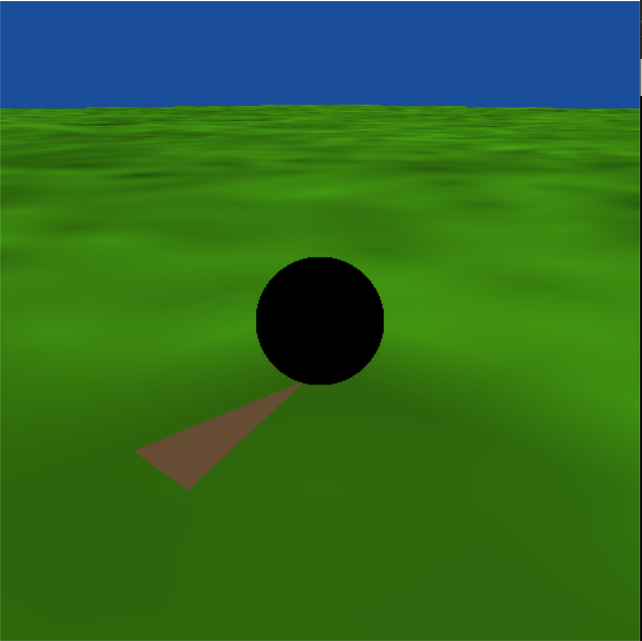
\includegraphics[width=5cm]{images/worksheet_3/low_tex_scale} }}%
	\qquad
	\subfloat[\centering High tex\_scale]{{
\includegraphics[width=5cm]{images/worksheet_3/tex_scale_10} }}%
	
	\caption{Comparison between High and Low tex\_scale}%
	\label{fig:tex_scale_comparison}%
\end{figure}
By implement an inverse sphere mapping we can calculate the uv-coordinates necessary to texture a sphere. The result can be seen in figure \ref{fig:textured_sphere} 
\begin{lstlisting}
void InvSphereMap::project_direction(const float3& d, float& u, float& v) const
{
	float3 ve = normalize(d);
	float teta = acos(ve.x);
	float fi = atan2(ve.y, ve.x);
	u = teta / M_PIf;
	v = fi / 2 * M_PIf;
}
\end{lstlisting}

\begin{figure}[H]
	\centering
	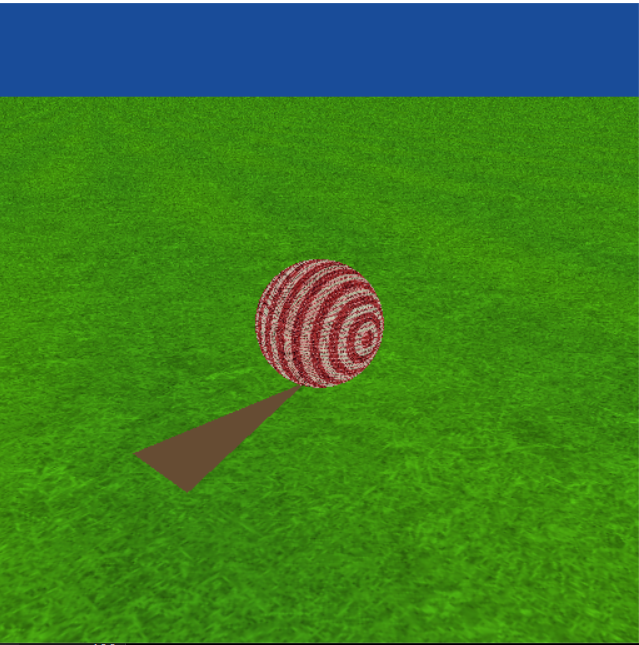
\includegraphics[scale=\imagescale]{images/worksheet_3/textured_sphere}
	\caption{Textured sphere}
	\label{fig:textured_sphere}
\end{figure}
	\section{Worksheet 4}
\subsection{Triangle Meshes}
We want to be able to render arbitrary surface. One way to do this is by using triangle meshes. We now load the Cornell box along with it's blocks instead of the default scene. The preview can be seen from figure \ref{fig:cornell_base_rendering}
\begin{figure}[H]
	\centering
	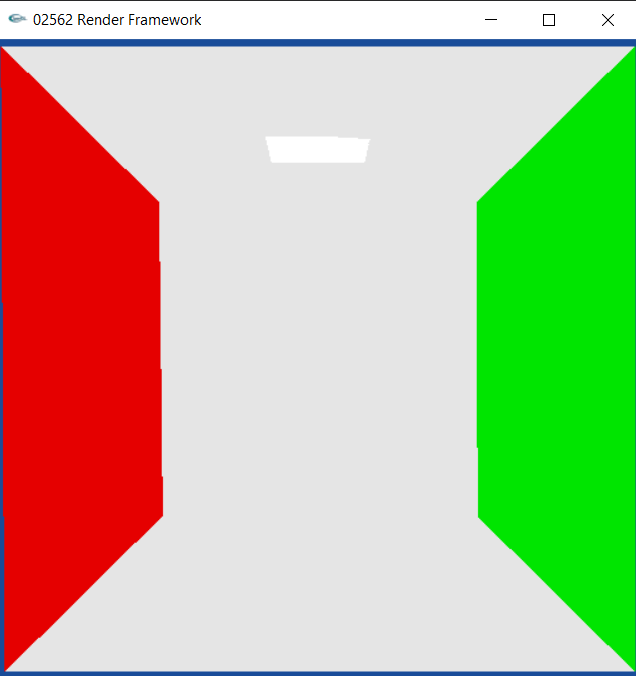
\includegraphics[scale=\imagescale]{images/worksheet_4/part_1}
	\caption{Cornell box base rendering}
	\label{fig:cornell_base_rendering}
\end{figure}
To implement ray tracing we have to implement the intersection function for the triangle meshes. This function is very similar to the intersection function for the triangles that we implemented on worksheet 1. The rendering obtained with ray tracing and base colours can be seen in figure \ref{fig:cornell_base_ray_tracing}.
\begin{lstlisting}
bool TriMesh::intersect(const Ray& r, HitInfo& hit, unsigned int prim_idx) const
{
	const uint3& face = geometry.face(prim_idx);
	const uint3& in_face = normals.face(prim_idx);
	float3 v0 = geometry.vertex(face.x);
	float3 v1 = geometry.vertex(face.y);
	float3 v2 = geometry.vertex(face.z);
	float3 n;
	float t;
	float v;
	float w;
	bool has_hit = ::intersect_triangle(r, v0, v1, v2, n, t, v, w);
	float u = 1.0f - v - w;
	
	if (has_hit) {
		hit.has_hit = true;
		hit.dist = t;
		hit.geometric_normal = -normalize(n);
		hit.shading_normal = hit.geometric_normal;
		
		hit.material = &materials[mat_idx[prim_idx]];
		hit.position = r.origin + r.direction * hit.dist;
	}
	return has_hit;
}
\end{lstlisting}

\begin{figure}[H]
	\centering
	
\includegraphics[scale=\imagescale]{images/worksheet_4/part_2}
	\caption{Cornell ray tracing base colour rendering}
	\label{fig:cornell_base_ray_tracing}
\end{figure}
The cornell box has an area light, to enable this source we have to implement the AreaLight::sample method.	
\begin{lstlisting}
bool AreaLight::sample(const float3& pos, float3& dir, float3& L) const
{
	const IndexedFaceSet& normals = mesh->normals;
	int n_faces = mesh->geometry.no_faces();
	float3 light_pos = mesh->compute_bbox().center();
	
	dir = light_pos - pos;
	float dir_norm = length(dir);
	dir = normalize(dir);
	
	float3 intensity = make_float3(0.0f);
	for (int i = 0; i < n_faces; i++) {
		uint3 face = mesh->geometry.face(i);
		float3 face_normal = normalize(normals.vertex(face.x) + normals.vertex(face.y) + normals.vertex(face.z));
		intensity = intensity + dot(-dir, face_normal) * get_emission(i) * mesh->face_areas[i];
	}
	
	float epsilon = 1e-4;
	float cutoff_distance = dir_norm - epsilon;
	Ray shadow_ray = Ray(pos, dir, 0, epsilon, dir_norm-epsilon);
	HitInfo hit_info = HitInfo();
	tracer->trace_to_any(shadow_ray, hit_info);
	
	if (!hit_info.has_hit) {
		L = intensity / (dir_norm * dir_norm);
	}
	return !hit_info.has_hit;
	
}
\end{lstlisting}

\begin{figure}[H]
	\centering
	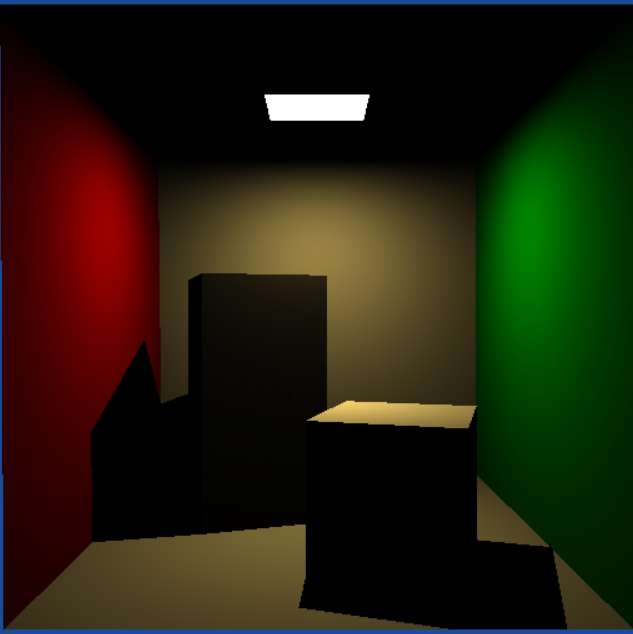
\includegraphics[scale=\imagescale]{images/worksheet_4/part3_after_rendering}
	\caption{Cornell Box with flat shading}
	\label{fig:cornell_lambertian_shading}
\end{figure}
We load now a different triangle mesh, the Utah teapot. The teapot is lit by a default directional light. To enable this source we have to implement then the function Directional::sample.
\begin{lstlisting}
bool Directional::sample(const float3& pos, float3& dir, float3& L) const
{
	dir = -light_dir;
	
	//Worksheet2 - point 1
	float epsilon = 1e-4;
	float cutoff_distance = RT_DEFAULT_MAX;
	
	Ray shadow_ray = Ray(pos, dir, 0, epsilon, RT_DEFAULT_MAX);
	HitInfo hit_info = HitInfo();
	
	tracer->trace_to_any(shadow_ray, hit_info);
	if (!hit_info.has_hit) {
		L = emission;
	}
	return !hit_info.has_hit;
}
\end{lstlisting}

\begin{figure}[H]
	\centering
	
\includegraphics[scale=\imagescale]{images/worksheet_4/part4_after_rendering}
	\caption{Utah teapot with flat shading}
	\label{fig:utah_lambertian}
\end{figure}
As we can see from figure \ref{fig:utah_lambertian} the result looks pretty blocky. This can be solved by using interpolation of vertex normals. We have to appropiately modify the intersect function of the Triangle Mesh that we made before.
\begin{lstlisting}
bool TriMesh::intersect(const Ray& r, HitInfo& hit, unsigned int prim_idx) const
{
	const uint3& face = geometry.face(prim_idx);
	const uint3& in_face = normals.face(prim_idx);
	float3 v0 = geometry.vertex(face.x);
	float3 v1 = geometry.vertex(face.y);
	float3 v2 = geometry.vertex(face.z);
	
	
	float3 n;
	float t;
	float v;
	float w;
	bool has_hit = ::intersect_triangle(r, v0, v1, v2, n, t, v, w);
	float u = 1.0f - v - w;
	
	if (has_hit) {
		hit.has_hit = true;
		hit.dist = t;
		hit.geometric_normal = -normalize(n);
		if (has_normals()) {
			hit.shading_normal = normalize(u * normals.vertex(in_face.x) + v * normals.vertex(in_face.y) + w * normals.vertex(in_face.z));
		}
		else {
			hit.shading_normal = hit.geometric_normal;
		}
		hit.material = &materials[mat_idx[prim_idx]];
		hit.position = r.origin + r.direction * hit.dist;
	}
	return has_hit;
}
\end{lstlisting}

\begin{figure}[H]
	\centering
	
\includegraphics[scale=\imagescale]{images/worksheet_4/part_5}
	\caption{Utah teapot with interpolation between normals}
	\label{fig:utah_interpolation}
\end{figure}
As we can see from figure \ref{fig:utah_interpolation} the result looks much better now.
\subsection{Space Subdivision}
To make the renderings of our polygons much faster we need to use a more efficient data structure to check for intersections.\\
We do this by using the given implementation of the BSP data structure. The main idea behind BSP trees is the fact that hyperplanes subdivide the 3-dimensional space in two. We start in a situation where our tree is formed by a single node containing all of the primitive polygons of our objects in the scene, then we chose the polygon contained in the hyperplane which best subdivides the scene. Now we modify our tree such that the root of our tree becomes the polygon related to the hyperplane we selected before and that  the left and right sub-nodes contain all of the polygons on one side and the other of the selected hyperplane. We repeat this recursevely for both of the subnodes of the tree.


\begin{lstlisting}
bool BspTree::closest_hit(Ray& r, HitInfo& hit) const
{
	closest_plane(r, hit);
	intersect_min_max(r);
	intersect_node(r,hit,*root);
	return hit.has_hit;
}

bool BspTree::any_hit(Ray& r, HitInfo& hit) const
{
	any_plane(r, hit);
	intersect_min_max(r);
	intersect_node(r, hit, *root);
	return hit.has_hit;
}
\end{lstlisting}

\begin{table}[H]
	\centering
	\begin{tabular}{|l|l|l|l|}
		\hline
		\textbf{}                       & \textbf{Number of Triangles} & \textbf{Default} & \textbf{BSP Tree} \\ \hline
		\textbf{Stanford Bunny}         & 69451                        & 337.853          & 0.15              \\ \hline
		\textbf{Utah Teapot}            & 6320                         & 22.449s          & 0.279s            \\ \hline
		\textbf{Cornell Box and Blocks} & 24                           & 0.205            & 0.086s            \\ \hline
	\end{tabular}
	\caption{Time comparison between our default data structure and the BSP Tree}
	\label{table:time_comparisons}
\end{table}
From table \ref{table:time_comparisons} we can see that with our default data structure the time complexity seems to increase linearly with the number of triangles of the polygon.\\
On the other with the BSP data structures it doesn't seem to be a linear relation between the time complexity and the number of triangles since the utah teapot takes almost double the time of the stanford bunny despite the fact it has a number of trinagles which is ten times lower.
Despite this the rendering times drop substantially in all of the cases.
	\section{Worksheet 5}
	\section{Worksheet 6}
\subsection{Anti-Aliasing}
The pixel subdivision level is increased with the key \textbf{+} and decreased with the key \textbf{-}.\\
The array jitters contains an array of two dimentionals vector, which are random displacements of the coordinates of the lower left corner of the pixel.\\
If we have a subdivision level $s$ then function compute\_jitters will generate $s^2$ jitters. 
To reomove the aliasing artifacts we modify the compute pixel function that we made some worksheets before so that it casts a ray through all the jittered position of the pixels and then we return the averaged color computed from all the jittered positions.
\begin{lstlisting}
float3 RayCaster::compute_pixel(unsigned int x, unsigned int y) const
{
	Camera* camera = scene->get_camera();
	float2 coords = make_float2(lower_left.x + win_to_ip.x * x, lower_left.y + win_to_ip.y * y);
	float3 color = make_float3(0.0f);
	
	for (int i = 0; i < jitter.size(); i++) {
		Ray ray = camera->get_ray(coords+jitter[i]);
		
		HitInfo hit = HitInfo();
		bool has_hit = scene->closest_hit(ray, hit);
		if (has_hit) {
			color=color+ get_shader(hit)->shade(ray, hit);
		}
		else {
			color = color + get_background(ray.direction);
		}
	}
	return color / jitter.size();
}
\end{lstlisting}
As we can see from table \ref{table:time_comparison}  the rendering time seems to increase linearly with the subdivision level.
\begin{table}[H]
	\centering
	\begin{tabular}{|l|l|}
		\hline
		\textbf{Subdivision Level} & \textbf{Rendering Time} \\ \hline
		\textbf{1}                 & 2.401s                  \\ \hline
		\textbf{4}                 & 8.994s                  \\ \hline
		\textbf{9}                 & 21.63s                  \\ \hline
		\textbf{16}                & 36.325s                 \\ \hline
	\end{tabular}
	\caption{Comparison between subdivision level and rendering times}
	\label{table:time_comparison}
\end{table}
From figure \ref{fig:subdivison_comparison} we can see the differences between a subdivision level of 1, 4 and 9 are pretty noticeable. However increasing even more the subdivision level doesn't seem to provide any noticeable difference.
\begin{figure}[H]
	\centering
	\subfloat[\centering Subdivision level 1]{{
\includegraphics[width=5cm]{images/worksheet_6/subdivision_1} }}%
	\qquad
	\subfloat[\centering Subdivision level 4]{{
\includegraphics[width=5cm]{images/worksheet_6/subdivision_4} }}%
	\qquad
	\subfloat[\centering Subdivision level 9]{{
\includegraphics[width=5cm]{images/worksheet_6/subdivision_9} }}%
	\qquad
	\subfloat[\centering Subdivision level 16]{{
\includegraphics[width=5cm]{images/worksheet_6/subdivision_16} }}%	
	
	\caption{Comparison between different subdivision levels}%
	\label{fig:subdivison_comparison}%
\end{figure}

\subsection{Progressive path tracing}
To enable indirect illumination we have to implement the functions optix::float3 sample\_cosine\_weighted and MCGlossy::shade.
\begin{lstlisting}
inline optix::float3 sample_cosine_weighted(const optix::float3& normal)
{
	//return optix::make_float3(0.0f);
	// Get random numbers
	double epsilon_1 = mt_random_half_open();
	double epsilon_2 = mt_random_half_open();
	// Calculate new direction as if the z-axis were the normal
	float teta = acos(sqrt(1 - epsilon_1));
	float phi = 2 * M_PIf * epsilon_2;
	optix::float3 w = optix::make_float3(cos(phi)*sin(teta),sin(phi)*sin(teta),cos(teta));
	// Rotate from z-axis to actual normal and return
	rotate_to_normal(normal,w);
	return w;
}

float3 MCGlossy::shade(const Ray& r, HitInfo& hit, bool emit) const
{
	if(hit.trace_depth >= max_depth)
	return make_float3(0.0f);
	float3 rho_d = get_diffuse(hit);
	float3 result = make_float3(0.0f);
	
	float probability = (rho_d.x + rho_d.y + rho_d.z) / 3;
	float epsilon = mt_random_half_open();
	float3 L_indirect = make_float3(0.0f);
	if (epsilon < probability) {
		float3 w_j = sample_cosine_weighted(hit.shading_normal);
		HitInfo indirect_hit;
		indirect_hit.trace_depth = hit.trace_depth + 1;
		Ray new_ray = Ray(hit.position, w_j, 0, pow(10,-4),RT_DEFAULT_MAX);
		tracer->trace_to_closest(new_ray,indirect_hit);
		L_indirect = rho_d * shade_new_ray(new_ray, indirect_hit, false);
		L_indirect = L_indirect / probability;
	}
	return result + Lambertian::shade(r,hit,emit)+L_indirect;
}
\end{lstlisting}
In figure \ref{fig:ambient_light} you can see a rendering of the conrnell box with ambient lighting and indirect illuminations obtained with 300 samples per pixels.	
\begin{figure}[H]
	\centering
	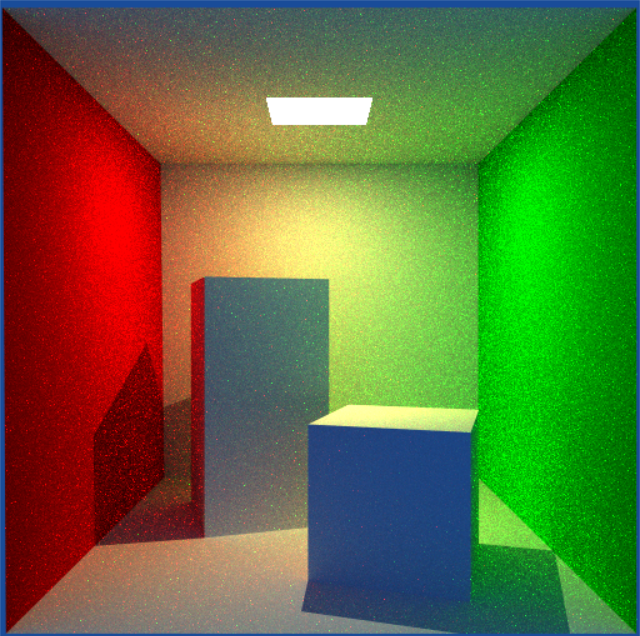
\includegraphics[scale=\imagescale]{images/worksheet_6/ambient_light}
	\caption{Cornell Box with indirect illumination}
	\label{fig:ambient_light}
\end{figure}
	\section{Worksheet 7}
\begin{lstlisting}
bool PointLight::emit(Ray& r, HitInfo& hit, float3& Phi) const
{
	float3 direction;
	do{
		direction.x = 2.0f * mt_random() - 1.0f;
		direction.y = 2.0f * mt_random() - 1.0f;
		direction.z = 2.0f * mt_random() - 1.0f;
	}while (dot(direction, direction) > 1.0f);
	direction = normalize(direction);
	r = Ray(light_pos, direction, 1,1e-4, RT_DEFAULT_MAX);
	
	// Trace ray
	tracer->trace_to_closest(r, hit);
	
	// If a surface was hit, compute Phi and return true
	if (hit.has_hit) {
		Phi = intensity*4*M_PIf;
	}
	return hit.has_hit;
}

void ParticleTracer::trace_particle(const Light* light, const unsigned int caustics_done)
{
	if(caustics_done)
		return;
	
	// Shoot a particle from the sampled source
	Ray r;
	HitInfo hit;
	float3 Phi;
	if (!light->emit(r, hit, Phi)|| !scene->is_specular(hit.material)) {
		return;
	}
	
	// Forward from all specular surfaces
	while(scene->is_specular(hit.material) && hit.trace_depth < 500){
		switch(hit.material->illum)
		{
		case 3:  // mirror materials
			{
				// Forward from mirror surfaces here
				return;
			}
			break;
		case 11: // absorbing volume
		case 12: // absorbing glossy volume
			{
				// Handle absorption here (Worksheet 8)
			}
		case 2:  // glossy materials
		case 4:  // transparent materials
			{
				Ray refracted;
				HitInfo hit_refracted;
				float probability;
				
				trace_refracted(r, hit, refracted, hit_refracted, probability);
				
				float epsilon = mt_random();
				if (epsilon < probability) {
					Ray reflected;
					HitInfo hit_reflected;
					trace_reflected(r, hit, reflected, hit_reflected);
					r = reflected;
					hit = hit_reflected;
				}
				else {
					r = refracted;
					hit = hit_refracted;
				}
				if (!hit.has_hit) {
					return;
				}
			}
			break;
		default: 
			return;
		}
	}
	caustics.store(Phi,hit.position,-r.direction);
}
\end{lstlisting}

\begin{figure}[H]
	\centering
	
\includegraphics[scale=\imagescale]{images/worksheet_7/caustics_preview}
	\caption{Caustics preview}
	\label{fig:caustics_preview}
\end{figure}

\begin{lstlisting}
float3 PhotonCaustics::shade(const Ray& r, HitInfo& hit, bool emit) const
{	
	float3 irradiance=tracer->caustics_irradiance(hit,max_dist,photons);
	float3 radiance = irradiance * rho_d / M_PIf;
	return Lambertian::shade(r, hit, emit)+ radiance;
}
\end{lstlisting}

\begin{figure}[H]
	\centering
	
\includegraphics[scale=\imagescale]{images/worksheet_7/caustics_full_illum}
	\caption{Caustics and full illumination}
	\label{fig:caustics_full_illum}
\end{figure}

\begin{figure}[H]
	\centering
	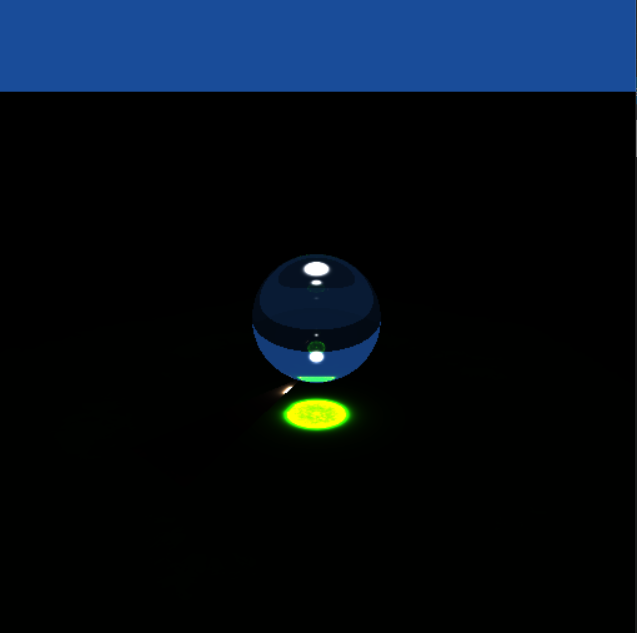
\includegraphics[scale=\imagescale]{images/worksheet_7/caustics_only}
	\caption{Caustics illumination only}
	\label{fig:caustics_only}
\end{figure}

	\section{Worksheet 8}
\subsection{Fresnel Reflectance}

\begin{lstlisting}
inline float fresnel_r_s(float cos_theta1, float cos_theta2, float ior1, float ior2)
{
	// Compute the perpendicularly polarized component of the Fresnel reflectance
	return (ior1 * cos_theta1 - ior2 * cos_theta2) / (ior1 * cos_theta1 + ior2 * cos_theta2);
}

inline float fresnel_r_p(float cos_theta1, float cos_theta2, float ior1, float ior2)
{
	// Compute the parallelly polarized component of the Fresnel reflectance
	
	return (ior2 * cos_theta2 - ior1 * cos_theta1) / (ior2 * cos_theta2 + ior1 * cos_theta1);
}

inline float fresnel_R(float cos_theta1, float cos_theta2, float ior1, float ior2)
{
	// Compute the Fresnel reflectance using fresnel_r_s(...) and fresnel_r_p(...)
	float r_s = fresnel_r_s( cos_theta1,  cos_theta2,  ior1,  ior2);
	float r_p= fresnel_r_p(cos_theta1, cos_theta2, ior1, ior2);
	
	return 0.5*(pow(r_s,2)+ pow(r_p, 2));
}
\end{lstlisting}

\begin{lstlisting}
bool RayTracer::trace_refracted(const Ray& in, const HitInfo& in_hit, Ray& out, HitInfo& out_hit, float& R) const
{
	float3 normal;
	float out_ior = get_ior_out(in, in_hit, normal);
	out_hit.ray_ior = out_ior;
	bool refraction = refract(out.direction, in.direction, normal, out_hit.ray_ior / in_hit.ray_ior);
	if (refraction) {
		out.origin = in_hit.position;
		out.tmin = 1e-4;
		out.tmax = RT_DEFAULT_MAX;
		out_hit.trace_depth = in_hit.trace_depth + 1;
		
		float cos_theta1 = dot(in.direction, in_hit.shading_normal);
		float cos_theta2 = dot(out.direction, in_hit.shading_normal);
		R = fresnel_R(cos_theta1, cos_theta2, in_hit.ray_ior, out_hit.ray_ior);
		
		trace_to_closest(out, out_hit);
	}
	else {
		R = 1;
	}
	
	return out_hit.has_hit;
}
\end{lstlisting}

\begin{figure}[H]
	\centering
	\subfloat[\centering R always set to 10\%]{{
\includegraphics[width=5cm]{images/worksheet_8/10_percent_fresnel} }}%
	\qquad
	\subfloat[\centering Fresnel reflectance]{{
\includegraphics[width=5cm]{images/worksheet_8/fresnel} }}%
	\captionsetup{justification=centering,margin=2cm}
	\caption{Comparison between default 10\% reflectance and fresnel reflectance (Fully transparent material)}%
	%\label{fig:tex_scale_comparison}%
\end{figure}

\begin{figure}[H]
	\centering
	\subfloat[\centering R always set to 10\%]{{
\includegraphics[width=5cm]{images/worksheet_2/part_5} }}%
	\qquad
	\subfloat[\centering Fresnel reflectance]{{
\includegraphics[width=5cm]{images/worksheet_8/default_scene_fresnel} }}%
	\captionsetup{justification=centering,margin=2cm}
	\caption{Comparison between default 10\% reflectance and fresnel reflectance (Glossy material)}%
	%\label{fig:tex_scale_comparison}%
\end{figure}

\begin{figure}[H]
	\centering
	\subfloat[\centering R always set to 10\%]{{
\includegraphics[width=5cm]{images/worksheet_7/caustics_preview} }}%
	\qquad
	\subfloat[\centering Fresnel reflectance]{{
\includegraphics[width=5cm]{images/worksheet_8/caustics_preview_fresnel} }}%
	\captionsetup{justification=centering,margin=2cm}
	\caption{Comparison between default 10\% reflectance and fresnel reflectance(White dots)}%
	%\label{fig:tex_scale_comparison}%
\end{figure}

\begin{figure}[H]
	\centering
	\subfloat[\centering R always set to 10\%]{{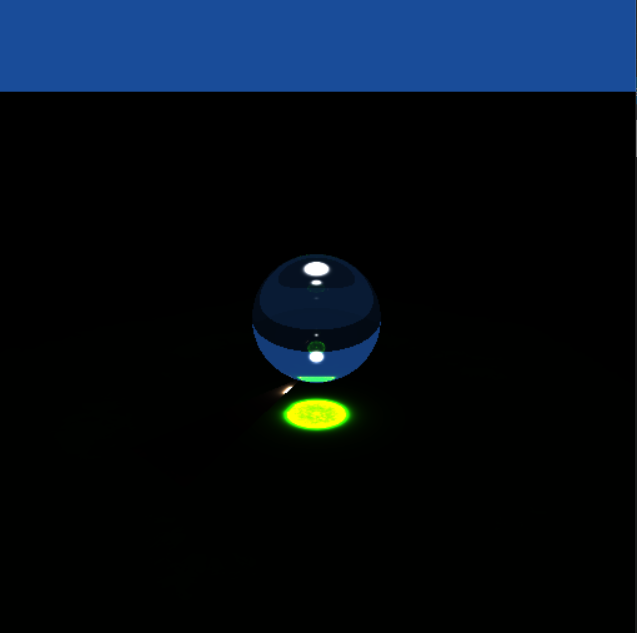
\includegraphics[width=5cm]{images/worksheet_7/caustics_only} }}%
	\qquad
	\subfloat[\centering Fresnel reflectance]{{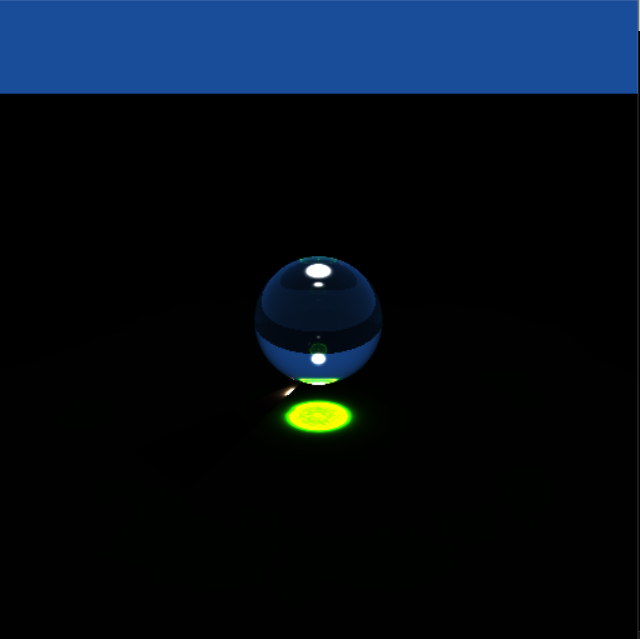
\includegraphics[width=5cm]{images/worksheet_8/caustics_only_fresnel} }}%
	\captionsetup{justification=centering,margin=2cm}
	\caption{Comparison between default 10\% reflectance and fresnel reflectance(Caustics only)}%
	%\label{fig:tex_scale_comparison}%
\end{figure}

\begin{figure}[H]
	\centering
	\subfloat[\centering R always set to 10\%]{{
\includegraphics[width=5cm]{images/worksheet_7/caustics_full_illum} }}%
	\qquad
	\subfloat[\centering Fresnel reflectance]{{
\includegraphics[width=5cm]{images/worksheet_8/caustics_full_illum_fresnel} }}%
	\captionsetup{justification=centering,margin=2cm}
	\caption{Comparison between default 10\% reflectance and fresnel reflectanace(Full illumination)}%
	%\label{fig:tex_scale_comparison}%
\end{figure}

\subsection{Absorbtion}

\begin{lstlisting}
float3 Volume::shade(const Ray& r, HitInfo& hit, bool emit) const
{
	// If inside the volume, Find the direct transmission through the volume by using
	// the transmittance to modify the result from the Transparent shader.
	float3 transmittance = get_transmittance(hit);
	return Transparent::shade(r, hit, emit)*transmittance;
}

float3 Volume::get_transmittance(const HitInfo& hit) const
{
	if(hit.material)
	{
		// Compute and return the transmittance using the diffuse reflectance of the material.
		// Diffuse reflectance rho_d does not make sense for a specular material, so we can use 
		// this material property as an absorption coefficient. Since absorption has an effect
		// opposite that of reflection, using 1/rho_d-1 makes it more intuitive for the user.
		float3 rho_d = make_float3(hit.material->diffuse[0], hit.material->diffuse[1], hit.material->diffuse[2]);
		float3 absorbtion= (1 / rho_d) - 1;
		float3 temp = -absorbtion * hit.dist;
		return make_float3(exp(temp.x), exp(temp.y), exp(temp.z));
	}
	return make_float3(1.0f);
}
\end{lstlisting}

\begin{lstlisting}
float3 GlossyVolume::shade(const Ray& r, HitInfo& hit, bool emit) const
{
	// Compute the specular part of the glossy shader and attenuate it
	// by the transmittance of the material if the ray is inside (as in
	// the volume shader).
	//return 0.9*Transparent::shade(r, hit, emit)+0.1*Mirror::shade(r, hit, emit)+Phong::shade(r, hit, emit);
	
	float3 rho_d = get_diffuse(hit);
	float3 rho_s = get_specular(hit);
	float s = get_shininess(hit);
	
	float3 phong_radiance = make_float3(0.0f);
	
	float3 wo = -r.direction;
	for (int i = 0; i < lights.size(); i++) {
		float3 wi;
		float3 L;
		bool shade = lights[i]->sample(hit.position, wi, L);
		float3 wr = reflect(wi, hit.shading_normal);
		if (dot(wi, hit.shading_normal) > 0) {
			float3 b = rho_s * (s + 2) / (2 * M_PIf);
			float c = pow(dot(wo, wr), s);
			float3 d = b * c;
			float3 e = L * dot(wi, hit.shading_normal);
			phong_radiance = phong_radiance + d * e;
		}
	}
	
	return 0.9 * Transparent::shade(r, hit, emit)+0.1*Mirror::shade(r, hit, emit)+ phong_radiance +Volume::shade(r, hit, emit);
}
\end{lstlisting}

\begin{lstlisting}
float3 ParticleTracer::get_transmittance(const HitInfo& hit) const
{
	if (hit.material)
	{
		// Compute and return the transmittance using the diffuse reflectance of the material.
		// Diffuse reflectance rho_d does not make sense for a specular material, so we can use 
		// this material property as an absorption coefficient. Since absorption has an effect
		// opposite that of reflection, using 1/rho_d-1 makes it more intuitive for the user.
		float3 rho_d = make_float3(hit.material->diffuse[0], hit.material->diffuse[1], hit.material->diffuse[2]);
		float3 absorbtion = (1 / rho_d) - 1;
		float3 temp = -absorbtion * hit.dist;
		return make_float3(exp(temp.x), exp(temp.y), exp(temp.z));
	}
	return make_float3(1.0f);   
}
\end{lstlisting}
Then we edit the case 12 of the switch case of the function ParticleTracer::trace\_particle in the following way.
\begin{lstlisting}
case 12: // absorbing glossy volume
{
	// Handle absorption here (Worksheet 8)
	if(dot(r.direction,hit.geometric_normal)>0)
	Phi = Phi* get_transmittance(hit);
}
\end{lstlisting}
\begin{figure}[H]
	\centering
	
\includegraphics[scale=\imagescale]{images/worksheet_8/final}
	\caption{Final rendering of the default scene}
	\label{fig:final_default}
\end{figure}
	\section{Worksheet 9}
\begin{lstlisting}
bool AreaLight::sample(const float3& pos, float3& dir, float3& L) const
{	
	const IndexedFaceSet& normals = mesh->normals;
	int n_faces = mesh->geometry.no_faces();
	
	uint3 random_triangle = mesh->geometry.face(rand() % n_faces);
	float xi_1 = mt_random();
	float xi_2 = mt_random();
	
	float u = 1 - sqrt(xi_1);
	float v = (1 - xi_2) * sqrt(xi_1);
	float w = xi_2 * sqrt(xi_1);
	
	float3 light_pos = u * mesh->geometry.vertex(random_triangle.x) + v * mesh->geometry.vertex(random_triangle.y) + w * mesh->geometry.vertex(random_triangle.z);
	//light_pos = mesh->compute_bbox().center();
	
	dir = light_pos - pos;
	float dir_norm = length(dir);
	dir = normalize(dir);
	
	float3 intensity = make_float3(0.0f);
	for (int i = 0; i < n_faces; i++) {
		uint3 face = mesh->geometry.face(i);
		float3 face_normal = normalize(normals.vertex(face.x) + normals.vertex(face.y) + normals.vertex(face.z));
		intensity = intensity + dot(-dir, face_normal) * get_emission(i) * mesh->face_areas[i];
	}
	
	float epsilon = 1e-4;
	float cutoff_distance = dir_norm - epsilon;
	Ray shadow_ray = Ray(pos, dir, 0, epsilon, dir_norm-epsilon);
	HitInfo hit_info = HitInfo();
	tracer->trace_to_any(shadow_ray, hit_info);
	
	if (!hit_info.has_hit) {
		L = intensity / (dir_norm * dir_norm);
	}
	return !hit_info.has_hit;
	
}
\end{lstlisting}

\begin{figure}[H]
	\centering
	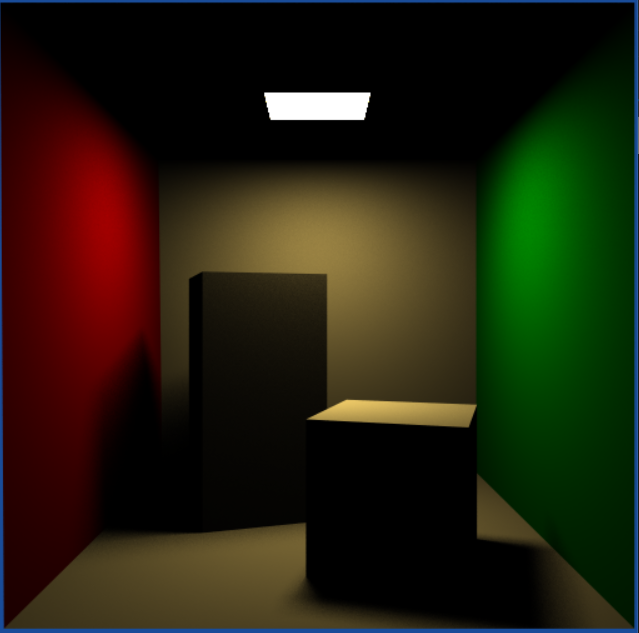
\includegraphics[scale=\imagescale]{images/worksheet_9/soft_shadow}
	\caption{Cornell box with soft shadows}
	\label{fig:cornell_soft_shadows}
\end{figure}

\begin{lstlisting}
float3 Holdout::shade(const Ray& r, HitInfo& hit, bool emit) const
{
	float ambient = 0.0f;
	for (int i = 0; i < samples; i++) {
		float3 dir = sample_cosine_weighted(hit.shading_normal);
		Ray new_ray = Ray(hit.position, dir, 0, 1e-4, RT_DEFAULT_MAX);
		HitInfo new_hit;
		tracer->trace_to_closest(new_ray,new_hit);
		if (!new_hit.has_hit)
		ambient = ambient + 1;
	}
	
	return ambient*tracer->get_background(r.direction);
}
\end{lstlisting}

\begin{figure}[H]
	\centering
	\subfloat[\centering Without holdout plane]{{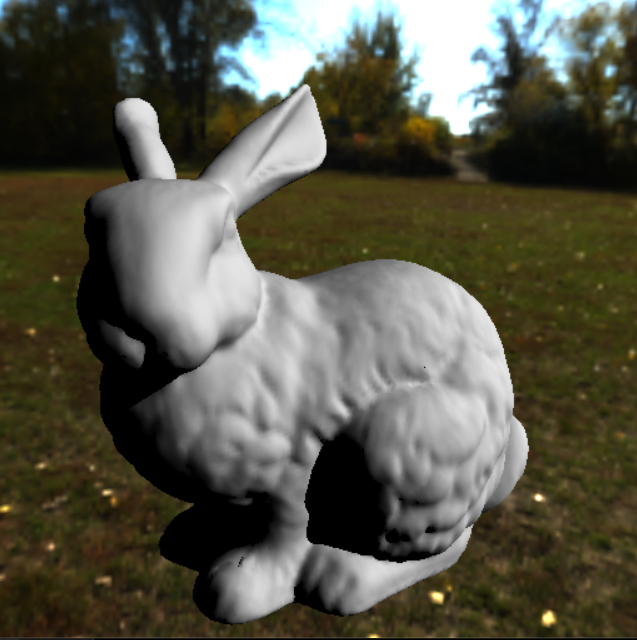
\includegraphics[width=5cm]{images/worksheet_9/bunny_no_holdout} }}%
	\qquad
	\subfloat[\centering With holdout plane]{{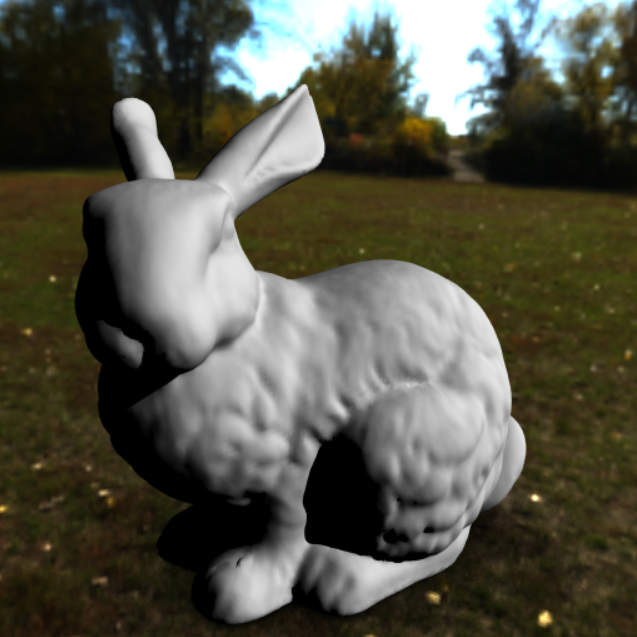
\includegraphics[width=5cm]{images/worksheet_9/bunny_soft_shadow} }}%
	
	\caption{Comparison of renderings of a bunny with and without an holdout plane}%
	\label{fig:holdout_comparison}%
\end{figure}

\begin{figure}[H]
	\centering
	\subfloat[\centering Without holdout plane]{{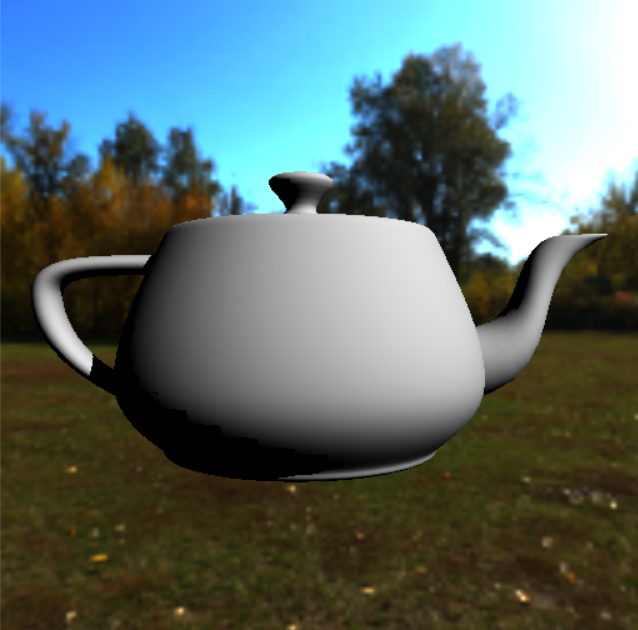
\includegraphics[width=5cm]{images/worksheet_9/teapot_no_holdout} }}%
	\qquad
	\subfloat[\centering With holdout plane]{{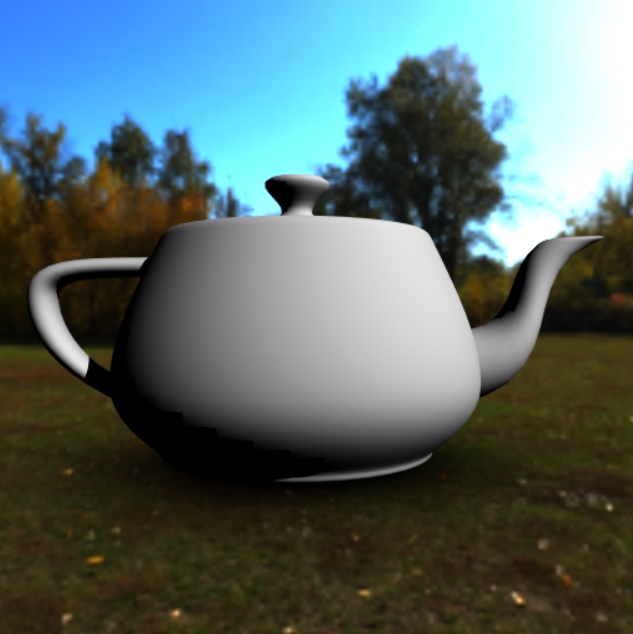
\includegraphics[width=5cm]{images/worksheet_9/teapot_soft_shadow} }}%
	
	\caption{Comparison of renderings of a teapot with and without an holdout plane}%
	\label{fig:holdout_comparison}%
\end{figure}
	\section{Project report}
In this section i'm going to 
As the project of this course i chose to re-implement some of the tecniques studied during the lectures in another framework based on opitx an API distribuited by NVIDIA which uses parallelization to reduce the rendering times.\\\\
I decided to follow the project initiator to make this project, so the first thing i did was building the framework with Cmake by following the procedure that was written in the project initiator. 
If we run it we get a rendering of a cow that can be seen in figure \ref{fig:cow}.
\begin{figure}[H]
	\centering
	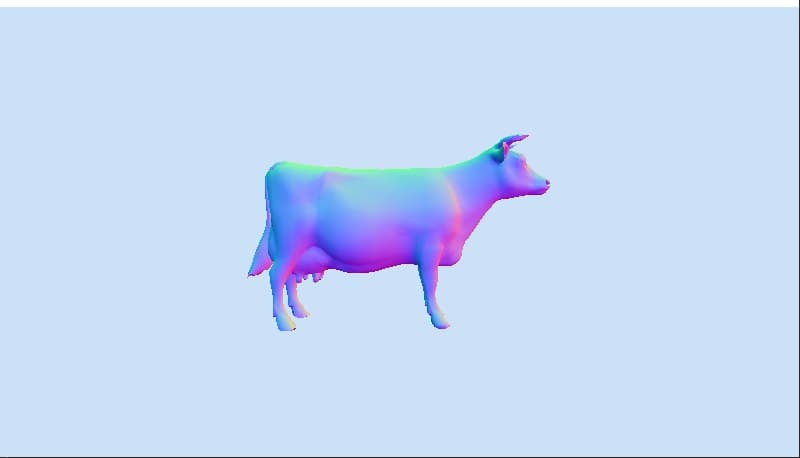
\includegraphics[scale=\imagescale]{images/project/1}
	\caption{}
	\label{fig:cow}
\end{figure}
Since we prefer using the famous stanford bunny for our tests we load this model instead.
\begin{figure}[H]
	\centering
	
\includegraphics[scale=\imagescale]{images/project/2}
	\caption{}
	\label{fig:bunny}
\end{figure}
Now we implement directional lighting by implementing the directional\_shading function inside the file contained directional\_shader.cu. The result can be seen in figure \ref{fig:directional_shadow}.
\begin{lstlisting}
RT_PROGRAM void directional_shader() 
{ 
	const float3& emission = Ka;
	const float3& rho_d = Kd;
	float3 normal = normalize(rtTransformNormal(RT_OBJECT_TO_WORLD, shading_normal)); 
	float3 ffnormal = faceforward(normal, -ray.direction, normal); 
	float3 color=make_float3(0,0,0);
	
	for(int i=0;i<lights.size();i++){
		color=color+(rho_d/3.14)*lights[i].emission*
			dot(lights[i].direction,ffnormal);
	}
	
	prd_radiance.result = color + emission; 
}
\end{lstlisting}

\begin{figure}[H]
	\centering
	
\includegraphics[scale=\imagescale]{images/project/3}
	\caption{Stanford bunny with directional shading}
	\label{fig:directional_shadow}
\end{figure}
Now we add shadows by implementing the function shadow\_shader contained in the file shadow\_shader.cu. The result can be seen in figure \ref{fig:shadow_shading}.
\begin{lstlisting}
RT_PROGRAM void shadow_shader() 
{ 
	#ifdef INDIRECT
	if(prd_radiance.depth > max_depth)
	{
		prd_radiance.result = make_float3(0.0f);
		return;
	}
	#endif
	float3 hit_pos = ray.origin + t_hit * ray.direction;
	float3 normal = normalize(rtTransformNormal(RT_OBJECT_TO_WORLD, shading_normal)); 
	float3 ffnormal = faceforward(normal, -ray.direction, normal); 
	const float3& emission = prd_radiance.emit ? Ka : make_float3(0.0f);
	const float3& rho_d = Kd;
	
	
	float3 color=make_float3(0,0,0);
	for(int i=0;i<lights.size();i++){
		Ray r=make_Ray(hit_pos,lights[i].direction,0,
			scene_epsilon,t_hit-scene_epsilon);
		PerRayData_radiance prd;
		rtTrace(top_shadower,r,prd);
		color=color+(rho_d/3.14)*prd.result*dot(lights[i].direction,ffnormal);
	}
	
	#ifdef INDIRECT
	// Indirect illumination
	uint& t = prd_radiance.seed;
	#endif
	
	prd_radiance.result = color + emission;
}
\end{lstlisting}

\begin{figure}[H]
	\centering
	
\includegraphics[scale=\imagescale]{images/project/4}
	\caption{Stanford bunny with shadow shading}
	\label{fig:shadow_shading}
\end{figure}
Now we load the cornell box along with the cornell blocks. Since the cornell box has an area light so we have to implement the appropiate shader.\\
Before implementing the area light shader we have to implement the sample\_center function first.
\begin{lstlisting}
__device__ __inline__ void sample_center(const float3& pos, float3& dir, float3& L, float& dist)
{
	float3 light_pos=make_float3(0.0f);
	
	for (int i = 0; i < light_verts.size(); i++) {
		light_pos = light_pos+light_verts[i];
	}
	light_pos = light_pos / light_verts.size();
	
	L = make_float3(0.0f);
	dir = normalize(light_pos - pos);
	dist = length(dir);
	
	float3 avg_normal = make_float3(0.0f);
	for (int i = 0; i < light_idxs.size(); i++) {
		float3 face_normal = normalize(light_norms[light_idxs[i].x] + light_norms[light_idxs[i].y] + light_norms[light_idxs[i].z]);
		avg_normal = face_normal + avg_normal;
		float3 a = light_verts[light_idxs[i].x];
		float3 b = light_verts[light_idxs[i].y];
		float3 c = light_verts[light_idxs[i].z];
		float face_area = (a.x*(b.y - c.y) + b.x*(c.y - a.y) + c.x*(a.y - b.y))/2;
		L = L + dot(-dir, face_normal)*light_emission*face_area;
	}
	avg_normal = avg_normal / light_idxs.size();
}
\end{lstlisting}
Now we can implement the area light shader which is basically only lambertian shading. The result can be seen in figure \ref{fig:area_light}.
\begin{lstlisting}
RT_PROGRAM void arealight_shader() 
{
	#ifdef INDIRECT
	if(prd_radiance.depth > max_depth)
	{
		prd_radiance.result = make_float3(0.0f);
		return;
	}
	#endif
	float3 hit_pos = ray.origin + t_hit * ray.direction;
	float3 normal = normalize(rtTransformNormal(RT_OBJECT_TO_WORLD, shading_normal)); 
	float3 ffnormal = faceforward(normal, -ray.direction, normal); 
	const float3& rho_d = Kd;
	uint& t = prd_radiance.seed;
	float3 color = prd_radiance.emit ? Ka : make_float3(0.0f);
	
	// Direct illumination
	float3 w_i;
	float3 L_e;
	float dist;
	sample_center(hit_pos, w_i, L_e, dist);

	
	Ray r=make_Ray(hit_pos,w_i,0,scene_epsilon,t_hit-scene_epsilon);
	PerRayData_radiance prd;
	rtTrace(top_shadower,r,prd);
	color=color+(rho_d/3.14)*prd.result*dot(w_i,ffnormal);
	
	//color+=rho_d;
	#ifdef INDIRECT
	// Indirect illumination
	#endif
	
	prd_radiance.result = color; 
}
\end{lstlisting}
As we can see from figure \ref{fig:area_light} the area light gets rendered correctly but the rest of the room doesn't seem to be rendered with the correct lighting.\\
Despite the multiple hours i spent trying fixing the problem i didn't manage to do it. However i think that the problem is in the shader and that the sampling function is implemented correctly.
\begin{figure}[H]
	\centering
	
\includegraphics[scale=\imagescale]{images/project/6}
	\caption{Cornell box and cornell blocks}
	\label{fig:area_light}
\end{figure}
If we load a pair of spheres instead of the CornellBoxes we can see that a second area light appears that previously was covered by the boxes. Such rendering can bee seen in figure \ref{fig:cornell_spheres}. We can notice that some weird shadows are being casted on the surfaces of the box, this is happens probably for the same reasons listed before.
\begin{figure}[H]
	\centering
	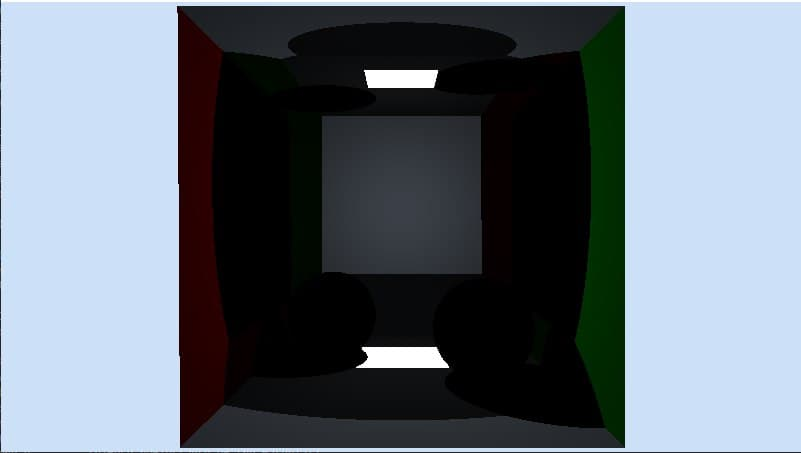
\includegraphics[scale=\imagescale]{images/project/7}
	\caption{Cornell box with spheres}
	\label{fig:cornell_spheres}
\end{figure}
The two spheres that can be seen in figure \ref{fig:cornell_spheres} are made of a transparent and mirror-like material. Since the shaders for this materials are not implemented yet for now they appear completly black. So to render them correcly we have to implement the appropiate shaders.\\
We start by implementing the mirror\_shader contained in the file mirror\_shader.cu
\begin{lstlisting}
RT_PROGRAM void mirror_shader()
{
	if(prd_radiance.depth > max_depth)
	{
		prd_radiance.result = make_float3(0.0f);
		return;
	}
	
	float3 hit_pos = ray.origin + t_hit * ray.direction;
	float3 normal = normalize(rtTransformNormal(RT_OBJECT_TO_WORLD, shading_normal));
	
	prd_radiance.result = make_float3(0.0f);
	if(prd_radiance.depth<=max_depth){
		float3 reflected_dir=reflect(ray.direction,shading_normal);
		PerRayData_radiance prd;
		float3 hit_pos=ray.direction*t_hit;
		Ray r=make_Ray(hit_pos,reflected_dir,0,scene_epsilon,RT_DEFAULT_MAX);
		rtTrace(top_object,r,prd_radiance);
		prd_radiance.depth+=1;
	}
}
\end{lstlisting}

\begin{figure}[H]
	\centering
	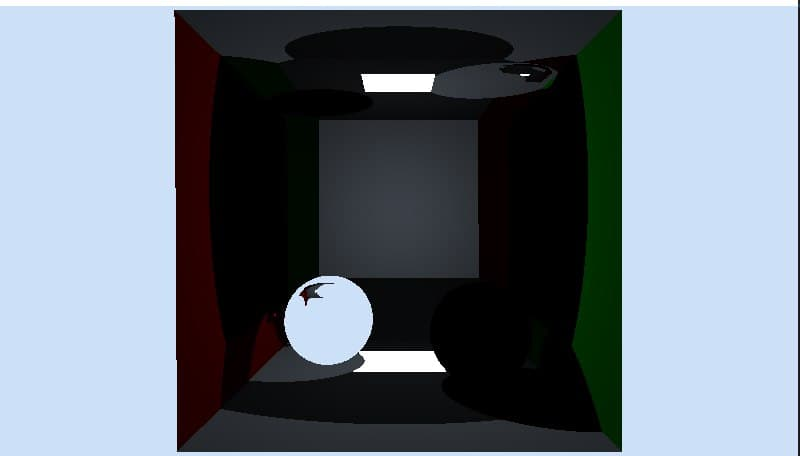
\includegraphics[scale=\imagescale]{images/project/9}
	\caption{Mirror sphere}
	\label{fig:mirror_ball}
\end{figure}
And then we do the same for the transparent\_shader function contained in the transparent\_shader.cu file.
\begin{lstlisting}
RT_PROGRAM void transparent_shader()
{
	if(prd_radiance.depth > max_depth)
	{
		prd_radiance.result = make_float3(0.0f);
		return;
	}
	
	float3 hit_pos = ray.origin + t_hit * ray.direction;
	float3 normal = normalize(rtTransformNormal(RT_OBJECT_TO_WORLD, shading_normal));
	float3 result = make_float3(0.0f);
	
	result=make_float3(0.0f);
	PerRayData_radiance out_prd;
	out_prd.depth=prd_radiance.depth-1;
	if(prd_radiance.depth<=max_depth){
		float3 reflected_dir=reflect(ray.direction,shading_normal);
		PerRayData_radiance prd;
		float3 hit_pos=ray.direction*t_hit;
		Ray reflect_r=make_Ray(hit_pos,reflected_dir,0,
			scene_epsilon,RT_DEFAULT_MAX);
		rtTrace(top_object,reflect_r,prd_radiance);
		prd_radiance.depth+=1;
		
		float3 refract_dir;
		bool refraction=refract(refract_dir,ray.direction,shading_normal,ior);
		Ray refract_r=make_Ray(hit_pos,refract_dir,0,scene_epsilon,RT_DEFAULT_MAX);
		rtTrace(top_object,reflect_r,prd_radiance);
		
		if(refraction){
			rtTrace(top_object,reflect_r,out_prd);
			out_prd.depth+=1;
		}	  
		
		
		float cos_theta=dot(ray.direction,shading_normal);
	}
	result=prd_radiance.result+out_prd.result;
	prd_radiance.result = result;
}
\end{lstlisting}

\begin{figure}[H]
	\centering
	\includegraphics[scale=\imagescale]{images/project/10}
	\caption{Transparent sphere}
	\label{fig:transparent_sphere}
\end{figure}
\end{document}
